\documentclass[journal,12pt,twocolumn]{IEEEtran}
\usepackage{amsmath,amssymb,amsfonts,amsthm}
\usepackage{txfonts}
\usepackage{tkz-euclide}
\usepackage{listings}
\usepackage{gvv}
\usepackage[latin1]{inputenc}
\usepackage{array}
\usepackage{pgf}
\usepackage{lmodern}

\begin{document}
\bibliographystyle{IEEEtran}

\title{DISCRETE 11.9.3 Q-4}
\author{EE23BTECH11066 - Yakkala Amarnath Karthik
}
\maketitle

\bibliographystyle{IEEEtran}
\textbf{Question:} \\ \\The $4^{th}$ term of a G.P. is square of its second term, and the first term is -3. Determine its $7^{th}$ term, and find the Z transform of the series.\\

\textbf{Solution:} \\ 
\begin{align}
 x(0)r^{3}=(x(0)r^{1})^2=x(0)^2r^2\\
r=x(0)=-3\\
(x\brak6)=x(0)r^{6}\\
x\brak6=\brak{-3}\brak{-3}^6=\brak{-3}^7\\
x(6)=-2187
\end{align}
  
Finding Z transform : \\
 
\begin{align}
    X \brak{z} & = \sum_{n=-\infty}^{\infty} x \brak{n}   z^{-n} \\
    & = \sum_{n=-\infty}^{\infty} ar^n  u \brak{n}   z^{-n} \\
    & = \sum_{n=0}^{\infty} ar^n  z^{-n} \\
    & = a( 1 + rz^{-1} + r^{2}z^{-2} +...)\\
    & = \frac{a}{{1 - rz^{-1}}} 
\end{align}
\hspace{3cm}\cbrak{ROC:|rz^{-1}|<1} \\
$X(n)=\frac{a}{1-rz^{-1}}= \frac{-3}{1+3z^{-1}}$.\\
\begin{figure}[ht]
        \centering
        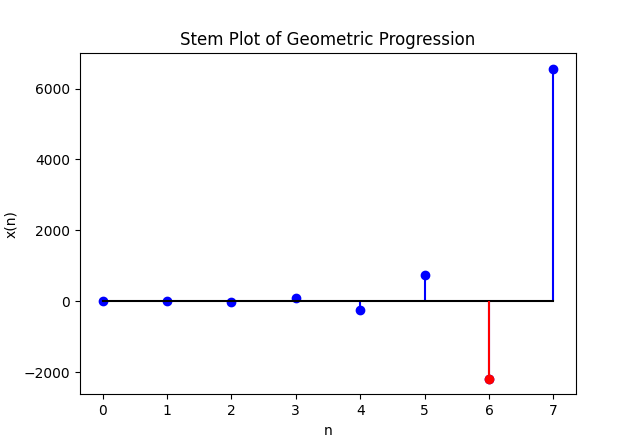
\includegraphics[width=0.45\textwidth]{stemplotfinal.jpeg}
        \centering
        \caption{Graph showing first 8 terms of the GP}
    \end{figure} \\
    
\begin{table}[ht]
  \centering
  \begin{tabular}{|c|c|c|}
    \hline
    \textbf{Variable} & \textbf{Description} & \textbf{value}\\
    \hline
    $x(0)$ & first term of G.P. & -3 \\
    \hline
    $r$ & Common ratio of G.P. & -3 \\
    \hline
    $x(n)$ & general term of the G.P. & $ar^{n}$ \\
    \hline
    -  & x\brak3=(x\brak1)^2 & -\\
    \hline
  \end{tabular}
  \caption{A Table with input parameters}
  \label{tab:1}
\end{table}


  \label{tab:1}
\end{table}
\end{document}
